\documentclass[10pt,aps,twocolumn,secnumarabic,balancelastpage,amsmath,amssymb,nofootinbib,floatfix]{revtex4}

%%\usepackage{setspace}
%%\setstretch{1.25}
\usepackage{graphicx}      % tools for importing graphics
%\usepackage{lgrind}        % convert program code listings to a form 
                            % includable in a LaTeX document
%\usepackage{xcolor}        % produces boxes or entire pages with 
                            % colored backgrounds
%\usepackage{longtable}     % helps with long table options
%\usepackage{epsf}          % old package handles encapsulated postscript issues
\usepackage{bm}            % special bold-math package. usge: \bm{mathsymbol}
%\usepackage{asymptote}     % For typesetting of mathematical illustrations
%\usepackage{thumbpdf}

\usepackage[colorlinks=true]{hyperref}  % this package should be added after 
                                        % all others.
                                        % usage: \url{http://web.mit.edu/8.13}

\renewcommand{\baselinestretch}{1.0} 

\begin{document}
\title{Measurement of the Free Fall Acceleration Using a Simple Pendulum}
\author{MIT Department of Physics}
\email{nodbody\@mit.edu}
\homepage{http://web.mit.edu/8.13/}
\date{\today}
%\affiliation{MIT Department of Physics}

%-------------------------------------------------------------------------------
\begin{abstract}
  The objective of this experiment is to measure the free fall acceleration using a pendulum. A pendulum will be constructed and measurements of its period will be performed. Using the small angle approximation the free fall acceleration will be determined. The simple experimental setup and execution will allow the experimenter to exercise all important ingredients for later experiments.
\end{abstract}

\maketitle

%-------------------------------------------------------------------------------
\section*{Preparatory questions}
There is not preparatory work required, except for remembering classical mechanics (8.01 or flavors of it).

%-------------------------------------------------------------------------------
\section{Introduction and Theory}

The pendulum is one of the classical examples used in the study of mechanics. When an object is suspended from a point and left to hang freely at a string, as shown in Figure~\ref{fig:pendulum} it will oscillate around the lowest position by a set frequency. Using Newton's Laws and realizing that only the force perpendicular to the string leads to a non-zero acceleration we find
%
\begin{equation}
  \vec{F} = m \vec{a} \ ; ~~ \to ~~ F_{\perp} = m g \sin\theta \ ,
\end{equation}
%
where $g$ denotes the free fall acceleration.
%
\begin{figure}[!h]
\centering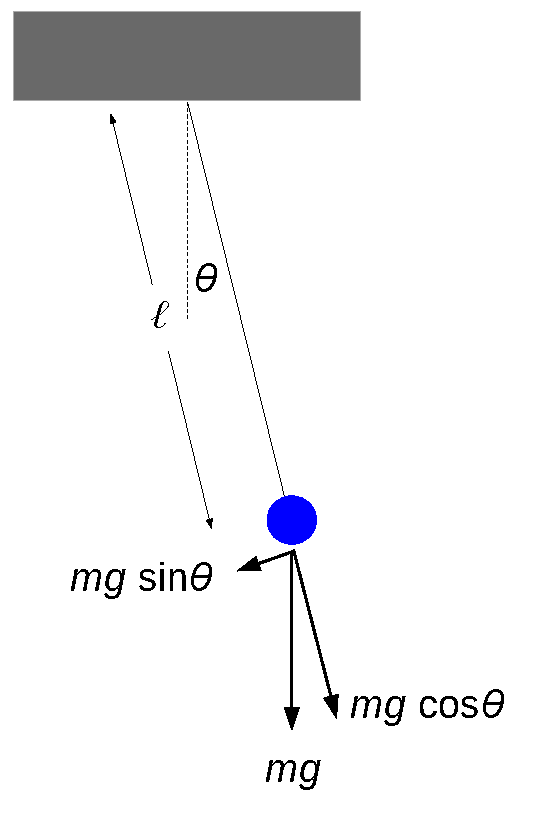
\includegraphics[width=0.2\textwidth]{figs/pendulum.pdf}
\caption{\label{fig:pendulum} Schematic drawing of simple pendulum showing forces on mass.}
\label{spend}
\end{figure}
%
Assuming that the angle of the displacement is small $\sin\theta \approx \theta$. This is a version of Hook's law if we replace the angular displacement with the real displacement $x_\perp = \ell \theta$ resulting in the following equation
%
\begin{equation}
  F_{\perp} = m\frac{g}{\ell} \ell\theta = m\frac{g}{\ell} x_\perp
  ~~\to~~
  m a_\perp = m\frac{g}{\ell} x_\perp \ .
\end{equation}
%
The differential equation for the displacement is solved and we find the solution as a function of time $t$ to be
%
\begin{equation}
  x_\perp = A \sin \left( \sqrt{ \frac{g}{\ell} } t - \phi \right) \ .
\end{equation}
%
The two parameters, A, for amplitude and, $\phi$, for phase, have to be determined by the initial condition of the system. For example, the size of the displacement and velocity of the pendulum have to be given at a time $t$.
%
When dividing the displacement by the length of the string we obtain the angular displacement and the corresponding equation of motion
%
\begin{equation}\label{eq:theta_of_t}
  \theta = \theta_\text{max} \sin \left( \sqrt{ \frac{g}{\ell} } t - \phi \right) \ ,
\end{equation}
%
where $\theta_{max}$ is the maximal angular displacement.

Given the above derivation it is important to note that the frequency and period of the pendulum are {\it independent} of the initial angular displacement amplitude, the phase and more importantly of the mass. The period $T$ for a simple pendulum, while not dependent on the mass, does depend on the length $\ell$ of the string and the value of the gravitational field strength $g$, according to
\begin{equation}\label{eq:period}
  T = 2 \pi \sqrt{\frac{\ell}{g}} \ .
\end{equation}
We can rewrite to solve for $g$ as
\begin{equation}
  g = 4 \pi^2 \frac{\ell}{T^2} \ .
\end{equation}

%-------------------------------------------------------------------------------
\section{Procedure}

\begin{itemize}
\item[1.] Obtain a string of length $\ell$ and a weight of mass $m$.
\item[2.] Measure the length of the pendulum to the middle of the pendulum bob.  Record the length of the pendulum.
\item[3.] Set the pendulum in motion until it completes $N$ complete oscillations, taking care to record this time. Then the period $T$ for one oscillation is just the number recorded divided by $N$.
\item[4.] Make a total of eight measurements for $g$ using two different masses at four different values for the length $\ell$.
\item[5.] Determine a mean value for $g$ and determine the uncertainty $\Delta g$ in the measurement.
\item[6.] Report $g \pm \Delta g$ and conclude.
\end{itemize}

%-------------------------------------------------------------------------------
\section{Investigating the Small Angle Approximation}

In deriving Equation~\ref{eq:theta_of_t} above, the small angle approximation $\sin\theta \approx \theta$ had been used. Here we want to investigate how the period in Equation~\ref{eq':period} is modified for oscillations at larger angles. Following Reference~\cite{cite:kidd-fogg}, we can approximate
\begin{equation} \label{eq:period-larger}
  T \approx 2 \pi \sqrt{\frac{\ell}{g \cos (\theta_\text{max}/2)}} \ ,
\end{equation}
for maximum angle $\theta_\text{max}$. Then,
\begin{equation}
  T = T_0 \left[ 1 + \frac{\theta_\text{max}^2}{16} + \frac{7 \theta_\text{max}^4}{1536} + .... \right] \ ,
\end{equation}
where $T_0 = 2 \pi \sqrt{\frac{\ell}{g}}$.

\begin{figure}[!h]
  \centering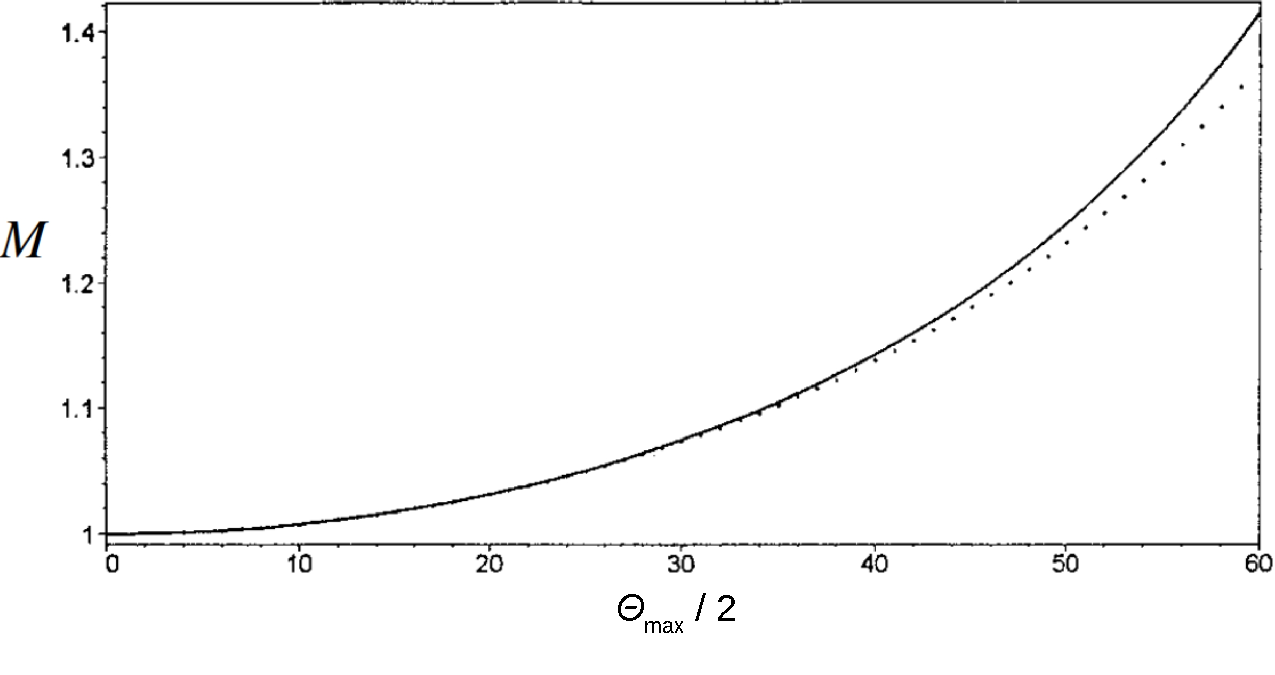
\includegraphics[width=0.4\textwidth]{figs/large-angle.pdf}
  \caption{\label{fig:period-larger} Exact value of $M=T/T_0$ (dotted curve) and the cosine approximation (solid curve) plotted against the angular half-amplitude.}
\end{figure}

Fix $\ell$ and $m$ and measure the period $T$ as a function of the starting angle $\theta_\text{max}$.  Plot the ratio of the measured period to the small angle approximation as a function of $\theta_\text{max}$. Compare to Equation~\ref{eq:period-larger} and Figure~\ref{fig:period-larger}.

Choose at least four different initial displacements and repeat each setup several times to obtain more accurate results. Make sure to go back to the last section and see whether the angle you chose for the experiment are not affected by this discrepancy. Quote the systematic uncertainty on $g$ due to this effect.

%-------------------------------------------------------------------------------
\section{Other uncertainties to consider}

There are a number of auxiliary measurements that have to be perfromed to setup and perform the complete experiment. There is the length of the pendulum, and the time for the
oscillations. Both have to be done carefully and various options should be considered.

Please, carefully propagate the uncertainty on period measurements and length measurements into your final result.

To reduce the uncertainty it is useful for each setup to make several measurements and average those. It is important to make sure those setups are reproducible as to not average values of different setups.

\subsection{Length of the pendulum}

The length of the pendulum has to be carefully determined. There are two points that are of importance: the suspension point and the bob itself. Also you have to consider the accuracy of the meter you are using.

Please, make sure to think about the bob. Does the size of the bob matter? You might want to try different sizes. Also is the derivation of the period correct for large bobs?

\subsection{Measurement of the time}

To measure the period one has to decide on a start and stop time. It is critical to define those times well. Which point of the trajectory is more precise, the point of maximal displacement or the point of highest velocity? Should you measure one period or several at once? As experimentalists it is best to think and then try. Can you improve your strategy and what is the resulting uncertainty?

Also, everybody today has cell phones, a recording might be even more precise.

\bibliography{pendulum-intro-experiment}

\end{document}
